% Generated by ArticleSignalDiagrams. Opaque vector fills only.
\documentclass[10pt,tikz,border=5pt]{standalone}
\usepackage{lmodern}
\usetikzlibrary{fit}
\begin{document}
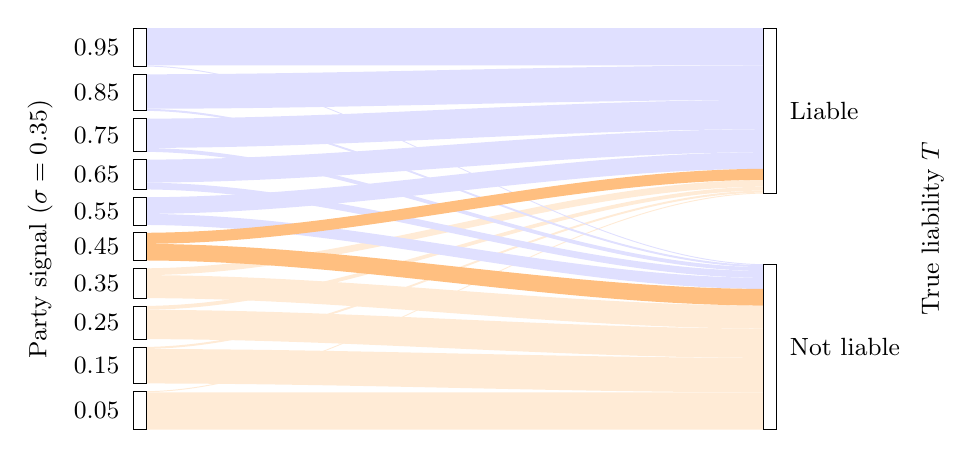
\begin{tikzpicture}[x=1cm,y=1cm,font=\small]\path[fill=orange!16!white,draw=none] (3.3,-5.1) .. controls (6,-5.1) and (8.6,-5.1) .. (11.3,-5.1) -- (11.3,-4.625459) .. controls (8.6,-4.625459) and (6,-4.625459) .. (3.3,-4.625459) -- cycle;
\path[fill=orange!16!white,draw=none] (3.3,-4.625459) .. controls (6,-4.625459) and (8.6,-2.1) .. (11.3,-2.1) -- (11.3,-2.087694) .. controls (8.6,-2.087694) and (6,-4.613152) .. (3.3,-4.613152) -- cycle;
\path[fill=orange!16!white,draw=none] (3.3,-4.513152) .. controls (6,-4.513152) and (8.6,-4.625459) .. (11.3,-4.625459) -- (11.3,-4.187908) .. controls (8.6,-4.187908) and (6,-4.075602) .. (3.3,-4.075602) -- cycle;
\path[fill=orange!16!white,draw=none] (3.3,-4.075602) .. controls (6,-4.075602) and (8.6,-2.087694) .. (11.3,-2.087694) -- (11.3,-2.062145) .. controls (8.6,-2.062145) and (6,-4.050053) .. (3.3,-4.050053) -- cycle;
\path[fill=orange!16!white,draw=none] (3.3,-3.950053) .. controls (6,-3.950053) and (8.6,-4.187908) .. (11.3,-4.187908) -- (11.3,-3.815915) .. controls (8.6,-3.815915) and (6,-3.57806) .. (3.3,-3.57806) -- cycle;
\path[fill=orange!16!white,draw=none] (3.3,-3.57806) .. controls (6,-3.57806) and (8.6,-2.062145) .. (11.3,-2.062145) -- (11.3,-2.01324) .. controls (8.6,-2.01324) and (6,-3.529156) .. (3.3,-3.529156) -- cycle;
\path[fill=orange!16!white,draw=none] (3.3,-3.429156) .. controls (6,-3.429156) and (8.6,-3.815915) .. (11.3,-3.815915) -- (11.3,-3.524311) .. controls (8.6,-3.524311) and (6,-3.137551) .. (3.3,-3.137551) -- cycle;
\path[fill=orange!16!white,draw=none] (3.3,-3.137551) .. controls (6,-3.137551) and (8.6,-2.01324) .. (11.3,-2.01324) -- (11.3,-1.926925) .. controls (8.6,-1.926925) and (6,-3.051236) .. (3.3,-3.051236) -- cycle;
\path[fill=blue!12!white,draw=none] (3.3,-2.5) .. controls (6,-2.5) and (8.6,-3.313541) .. (11.3,-3.313541) -- (11.3,-3.173075) .. controls (8.6,-3.173075) and (6,-2.359533) .. (3.3,-2.359533) -- cycle;
\path[fill=blue!12!white,draw=none] (3.3,-2.359533) .. controls (6,-2.359533) and (8.6,-1.786459) .. (11.3,-1.786459) -- (11.3,-1.575689) .. controls (8.6,-1.575689) and (6,-2.148764) .. (3.3,-2.148764) -- cycle;
\path[fill=blue!12!white,draw=none] (3.3,-2.048764) .. controls (6,-2.048764) and (8.6,-3.173075) .. (11.3,-3.173075) -- (11.3,-3.08676) .. controls (8.6,-3.08676) and (6,-1.962449) .. (3.3,-1.962449) -- cycle;
\path[fill=blue!12!white,draw=none] (3.3,-1.962449) .. controls (6,-1.962449) and (8.6,-1.575689) .. (11.3,-1.575689) -- (11.3,-1.284085) .. controls (8.6,-1.284085) and (6,-1.670844) .. (3.3,-1.670844) -- cycle;
\path[fill=blue!12!white,draw=none] (3.3,-1.570844) .. controls (6,-1.570844) and (8.6,-3.08676) .. (11.3,-3.08676) -- (11.3,-3.037855) .. controls (8.6,-3.037855) and (6,-1.52194) .. (3.3,-1.52194) -- cycle;
\path[fill=blue!12!white,draw=none] (3.3,-1.52194) .. controls (6,-1.52194) and (8.6,-1.284085) .. (11.3,-1.284085) -- (11.3,-0.912092) .. controls (8.6,-0.912092) and (6,-1.149947) .. (3.3,-1.149947) -- cycle;
\path[fill=blue!12!white,draw=none] (3.3,-1.049947) .. controls (6,-1.049947) and (8.6,-3.037855) .. (11.3,-3.037855) -- (11.3,-3.012306) .. controls (8.6,-3.012306) and (6,-1.024398) .. (3.3,-1.024398) -- cycle;
\path[fill=blue!12!white,draw=none] (3.3,-1.024398) .. controls (6,-1.024398) and (8.6,-0.912092) .. (11.3,-0.912092) -- (11.3,-0.474541) .. controls (8.6,-0.474541) and (6,-0.586848) .. (3.3,-0.586848) -- cycle;
\path[fill=blue!12!white,draw=none] (3.3,-0.486848) .. controls (6,-0.486848) and (8.6,-3.012306) .. (11.3,-3.012306) -- (11.3,-3) .. controls (8.6,-3) and (6,-0.474541) .. (3.3,-0.474541) -- cycle;
\path[fill=blue!12!white,draw=none] (3.3,-0.474541) .. controls (6,-0.474541) and (8.6,-0.474541) .. (11.3,-0.474541) -- (11.3,-0) .. controls (8.6,-0) and (6,-0) .. (3.3,-0) -- cycle;
\path[fill=orange!50!white,draw=none] (3.3,-2.951236) .. controls (6,-2.951236) and (8.6,-3.524311) .. (11.3,-3.524311) -- (11.3,-3.313541) .. controls (8.6,-3.313541) and (6,-2.740467) .. (3.3,-2.740467) -- cycle;
\path[fill=orange!50!white,draw=none] (3.3,-2.740467) .. controls (6,-2.740467) and (8.6,-1.926925) .. (11.3,-1.926925) -- (11.3,-1.786459) .. controls (8.6,-1.786459) and (6,-2.6) .. (3.3,-2.6) -- cycle;
\coordinate (axis-midline-0) at (0,-2.55);
\path[fill=white,draw=black,line width=0.3pt] (3.22,-5.1) rectangle (3.38,-4.613152);
\node[anchor=east,fill=white,inner sep=2pt] (bucket-0-0-0) at (3.12,-4.856576) {0.05};
\path[fill=white,draw=black,line width=0.3pt] (3.22,-4.513152) rectangle (3.38,-4.050053);
\node[anchor=east,fill=white,inner sep=2pt] (bucket-0-0-1) at (3.12,-4.281603) {0.15};
\path[fill=white,draw=black,line width=0.3pt] (3.22,-3.950053) rectangle (3.38,-3.529156);
\node[anchor=east,fill=white,inner sep=2pt] (bucket-0-0-2) at (3.12,-3.739605) {0.25};
\path[fill=white,draw=black,line width=0.3pt] (3.22,-3.429156) rectangle (3.38,-3.051236);
\node[anchor=east,fill=white,inner sep=2pt] (bucket-0-0-3) at (3.12,-3.240196) {0.35};
\path[fill=white,draw=black,line width=0.3pt] (3.22,-2.951236) rectangle (3.38,-2.6);
\node[anchor=east,fill=white,inner sep=2pt] (bucket-0-0-4) at (3.12,-2.775618) {0.45};
\path[fill=white,draw=black,line width=0.3pt] (3.22,-2.5) rectangle (3.38,-2.148764);
\node[anchor=east,fill=white,inner sep=2pt] (bucket-0-0-5) at (3.12,-2.324382) {0.55};
\path[fill=white,draw=black,line width=0.3pt] (3.22,-2.048764) rectangle (3.38,-1.670844);
\node[anchor=east,fill=white,inner sep=2pt] (bucket-0-0-6) at (3.12,-1.859804) {0.65};
\path[fill=white,draw=black,line width=0.3pt] (3.22,-1.570844) rectangle (3.38,-1.149947);
\node[anchor=east,fill=white,inner sep=2pt] (bucket-0-0-7) at (3.12,-1.360395) {0.75};
\path[fill=white,draw=black,line width=0.3pt] (3.22,-1.049947) rectangle (3.38,-0.586848);
\node[anchor=east,fill=white,inner sep=2pt] (bucket-0-0-8) at (3.12,-0.818397) {0.85};
\path[fill=white,draw=black,line width=0.3pt] (3.22,-0.486848) rectangle (3.38,-0);
\node[anchor=east,fill=white,inner sep=2pt] (bucket-0-0-9) at (3.12,-0.243424) {0.95};
\node[fit=(bucket-0-0-0) (bucket-0-0-1) (bucket-0-0-2) (bucket-0-0-3) (bucket-0-0-4) (bucket-0-0-5) (bucket-0-0-6) (bucket-0-0-7) (bucket-0-0-8) (bucket-0-0-9),inner sep=0pt] (source-labels-0) {};
\coordinate (axis-title-0-0) at (source-labels-0.west |- axis-midline-0);
\node[rotate=90,anchor=south,inner sep=0pt] at ([xshift=-0.18cm]axis-title-0-0) {Party signal ($\sigma=0.35$)};
\path[fill=white,draw=black,line width=0.3pt] (11.22,-5.1) rectangle (11.38,-3);
\node[anchor=west,fill=white,inner sep=2pt] (bucket-0-1-0) at (11.48,-4.05) {Not liable};
\path[fill=white,draw=black,line width=0.3pt] (11.22,-2.1) rectangle (11.38,-0);
\node[anchor=west,fill=white,inner sep=2pt] (bucket-0-1-1) at (11.48,-1.05) {Liable};
\node[fit=(bucket-0-1-0) (bucket-0-1-1),inner sep=0pt] (destination-labels-0) {};
\coordinate (axis-title-0-1) at (destination-labels-0.east |- axis-midline-0);
\node[rotate=90,anchor=north,inner sep=0pt] at ([xshift=0.18cm]axis-title-0-1) {True liability $T$};
\end{tikzpicture}
\end{document}

